% Um apêndice é algum conteúdo adicional de sua autoria que faz parte e
% colabora com a ideia geral do texto mas que, por alguma razão, não precisa
% fazer parte da sequência do discurso; por exemplo, a demonstração de um
% teorema intermediário, as perguntas usadas em uma pesquisa qualitativa etc.
%
% Um anexo é um documento que não faz parte da tese (em geral, nem é de sua
% autoria) mas é relevante para o conteúdo; por exemplo, a especificação do
% padrão técnico ou a legislação que o trabalho discute, um artigo de jornal
% apresentando a percepção do público sobre o tema da tese etc.
%
% Os comandos appendix e annex reiniciam a numeração de capítulos e passam
% a numerá-los com letras. "annex" não faz parte de nenhuma classe padrão,
% foi criado para este modelo. Se o trabalho não tiver apêndices ou anexos,
% remova estas linhas.
%
% Diferentemente de \mainmatter, \backmatter etc., \appendix e \annex não
% forçam o início de uma nova página. Em geral isso não é importante, pois
% o comando seguinte costuma ser "\chapter", mas pode causar problemas com
% a formatação dos cabeçalhos. Assim, vamos forçar uma nova página antes
% de cada um deles.

%%%% Apêndices %%%%

\makeatletter
\if@openright\cleardoublepage\else\clearpage\fi
\makeatother

\pagestyle{appendix}

\appendix

% \addappheadtotoc acrescenta a palavra "Apêndice" ao sumário; se
% só há apêndices, sem anexos, provavelmente não é necessário.
\addappheadtotoc

\chapter{Problemas-modelo para as simulações}\label{apendice:problemas-modelo}

Para testar os métodos numéricos e os resultados teóricos apresentados utilizamos dez conjuntos de valores iniciais, alguns obtidos na literatura e outros sorteados utilizando o método da seção \ref{secao:valores_iniciais}.

O problema-modelo \ref{probmodelo:lemniscata} é um problema planar de três corpos com trajetórias periódicas e coincidentes, na forma de uma lemniscata. Por sua periodicidade e coincidência de órbitas, permite fácil validação de integradores de baixa ordem, tendo sido utilizado com esse propósito.

O segundo problema-modelo (\ref{probmodelo:iau25}) foi um conjunto de valores amplamente utilizados no início das simulações numéricas do PNCG, tomado como o padrão internacional para que as simulações de diferentes pesquisadores pudessem ser comparadas. Trata-se de um problema de 25 corpos com massas iguais e que somam 1, velocidades nulas e com energia total $E=-0.2$. Os valores iniciais foram obtidos em \cite{Lecar1968}.

Todos os outros problemas foram utilizados na seção \ref{secao:simulacao_dinamica_de_formas} para verificar o comportamento da complexidade com diferentes valores de $N$ e de $E$. Os problemas com $N \geq 20$ não têm todas as suas coordenadas apresentadas devido à grande quantidade de números, mas constam no repositório \href{https://github.com/Potalej/gravidade-fortran}{https://github.com/potalej/gravidade-fortran} \citep{potalej_gravidade-fortran}.

\begin{probmodelo}[Lemniscata, \cite{Chenciner2000}]\label{probmodelo:lemniscata}
    Massas $m_i = 1$, $i=1,2,3$. Posições e momentos na tabela \ref{tab:lemniscata}.
    \begin{table}[H]
    \begin{tabular}{S[table-format=1.8, round-precision=8]|S[table-format=1.8, round-precision=8]}
    \multicolumn{1}{c}{$\vet x$} & \multicolumn{1}{c}{$\vet y$} \\
    \hline
        -0.97000436 &  0.24308753  \\
        -0.0        &  0.0  \\
         0.97000436 & -0.24308753  \\
    \hline
    \end{tabular}
    \quad
    \begin{tabular}{S[table-format=1.9, round-precision=9]|S[table-format=1.9, round-precision=9]}
    \multicolumn{1}{c}{$\vet p_x$} & \multicolumn{1}{c}{$\vet p_y$} \\
    \hline
         0.466203685 &  0.4323657300 \\
        -0.93240737  & -0.86473146   \\
         0.466203685 &  0.4323657300 \\
    \hline
    \end{tabular}
    \caption{Posições iniciais para o problema-modelo \ref{probmodelo:lemniscata}.}
    \label{tab:lemniscata}
\end{table}
\end{probmodelo}

\begin{probmodelo}[IAU-25, \cite{Lecar1968}]\label{probmodelo:iau25} 
    Massas $m_i = 0.04$, $i=1,2,...,25$. Momentos $\vet p_i = \vet 0$, $i=1,2,...,25$. Posições na tabela \ref{tab:iau25_lecar}.
    \begin{table}[H]
    \begin{tabular}{S|S|S}
    \multicolumn{1}{c}{$\vet X$} & \multicolumn{1}{c}{$\vet Y$} & \multicolumn{1}{c}{$\vet Z$} \\
    \hline
    -1.435339019209158  & -1.196080394997535   & -1.040917038416441 \\
    -1.600918225633380  & -1.433268456869804   & -0.3203325578291813    \\
    -0.6682692693377202 & -1.832619614531054   &  1.756554637456205 \\
    -1.006329727108562  & -0.4420086005314779  & -1.306648988044901 \\
    -1.286199985796732  & -0.5936998210709894  &  0.02911598953992680 \\
    -1.709740886338909  & -0.6341243127807427  &  1.710155177057028 \\
    -1.515429718153350  &  1.499840949607274   & -0.9165560967404586    \\
    -1.757994153161709  &  0.5824981279415633  & -0.5439513791077954    \\
    -1.020858179668266  &  1.245432523846089   &  0.6230107693204201    \\
     0.3623578617252796 & -1.462639856791440   & -1.347056225699700 \\
    -0.2618528693473776 & -1.180490198065629   &  0.2407017637492819    \\
     0.6764824947854864 & -1.535988122836920   &  0.7148086953996702    \\
     0.6975692665009510 &  0.5492508713153734  & -1.074140283549997 \\
    -0.2388485232971104 & -0.5528089412016879  &  0.07677338108658142 \\
    -0.3928864394947292 & -0.2839307266676437  &  1.407080127300226 \\
     0.3589534492431743 &  1.702937103980398   & -0.8184139363588995    \\
    -0.1150350974819667 &  1.801143445601472   & -0.1213591805860549    \\
     2.000302840973827  & -1.480587313284738   & -0.5041596816100792    \\
     1.414320895755169  & -0.3328032362360006  & -1.775193856401200 \\
     1.376012818146675  & -0.4872759065570369  &  0.07667511467777969 \\
     1.944710516217794  &  0.1861730047015689  &  1.424211414126600 \\
     1.009640791981309  &  1.200947609911347   & -1.909264265180262 \\
     1.659027755713092  &  1.014111792274731   &  0.2545976317092354    \\
     1.138161643051515  &  1.854946769972046   &  1.688446759524286 \\
     0.3721617599346991 &  1.8110433032708357  &  1.6758620285777291    \\
    \hline
    \end{tabular}
    \caption{Posições iniciais para o problema-modelo \ref{probmodelo:iau25}.}
    \label{tab:iau25_lecar}
\end{table}
\end{probmodelo}

\begin{probmodelo}[3 Corpos e constantes nulas]\label{probmodelo:3corpos_energia_nula}
    Massas $m_1 = m_2 = m_3 = 1$, posições e momentos lineares na tabela \ref{tab:3corpos_energia0}.
    \begin{table}[H]
    \begin{tabular}{S[table-format=1.8, round-precision=8]|S[table-format=1.8, round-precision=8]}
    \multicolumn{1}{c}{$\vet x$} & \multicolumn{1}{c}{$\vet y$} \\
    \hline
        -0.97000436 &  0.24308753 \\
        0.0         &  0.0        \\
        0.97000436  & -0.24308753 \\
    \hline
    \end{tabular}
    \quad
    \begin{tabular}{S[table-format=1.9, round-precision=9]|S[table-format=1.9, round-precision=9]}
    \multicolumn{1}{c}{$\vet p_x$} & \multicolumn{1}{c}{$\vet p_y$} \\
    \hline
         0.65552612 &  0.60794678 \\
        -1.31105225 & -1.21589357 \\
         0.79613551 &  0.60794678 \\
    \hline
    \end{tabular}
    \caption{Posições e velocidades iniciais para o problema-modelo \ref{probmodelo:3corpos_energia_nula}.}
    \label{tab:3corpos_energia0}
\end{table}    
\end{probmodelo}

\begin{probmodelo}[3 Corpos, constantes nulas exceto $E>0$]\label{probmodelo:3corpos_energia_positiva}
    Massas $m_1 = m_2 = m_3 = 1$, posições e momentos lineares na tabela \ref{tab:3corpos_energiapositiva}
    \begin{table}[H]
    \begin{tabular}{S[table-format=1.8, round-precision=8]|S[table-format=1.8, round-precision=8]}
    \multicolumn{1}{c}{$\vet x$} & \multicolumn{1}{c}{$\vet y$} \\
    \hline
        -1.11290666 & -0.10354093 \\
         0.0        &  0.76488086 \\
         1.11290666 & -0.66133993 \\
    \hline
    \end{tabular}
    \quad
    \begin{tabular}{S[table-format=1.9, round-precision=9]|S[table-format=1.9, round-precision=9]}
    \multicolumn{1}{c}{$\vet p_x$} & \multicolumn{1}{c}{$\vet p_y$} \\
    \hline
         0.53645589 &  1.06454049 \\
        -0.96477633 & -1.16156992 \\
         0.42832044 &  0.09702943 \\
    \hline
    \end{tabular}
    \caption{Posições e velocidades iniciais para o problema-modelo \ref{probmodelo:3corpos_energia_positiva}.}
    \label{tab:3corpos_energiapositiva}
\end{table}
\end{probmodelo}

\begin{probmodelo}[20 corpos]\label{probmodelo:20corpos_energia0}
    Trata-se de um problema com $N=20$, todas as integrais primeiras nulas e massas diferentes. As posições e momentos lineares podem ser visualizados na figura \ref{fig:probmodelo_20corpos}.
    \begin{figure}[H]
        \centering
        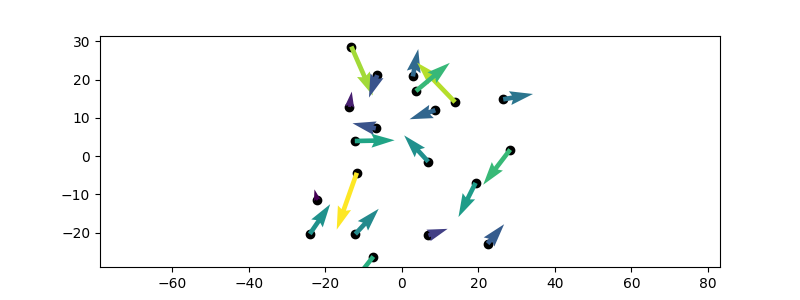
\includegraphics[width=0.5\linewidth]{tcc//img/20corpos_E_nula.png}
        \caption{Posições e momentos do problema-modelo \ref{probmodelo:20corpos_energia0}.}
        \label{fig:probmodelo_20corpos}
    \end{figure}
\end{probmodelo}

\begin{probmodelo}[100 corpos]\label{probmodelo:100corpos_energia0}
    Trata-se de um problema com $N=10^2$, todas as integrais primeiras nulas e massas iguais a $10^{-2}$. As posições e momentos lineares podem ser visualizados na figura \ref{fig:probmodelo_100corpos}.
    \begin{figure}[H]
        \centering
        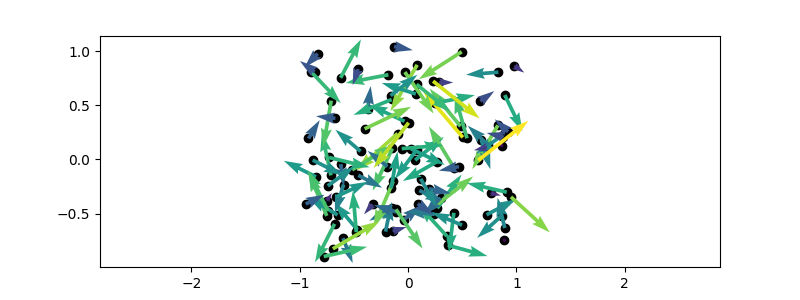
\includegraphics[width=0.5\linewidth]{tcc//img/100corpos_E_nula.png}
        \caption{Posições e momentos do problema-modelo \ref{probmodelo:100corpos_energia0}.}
        \label{fig:probmodelo_100corpos}
    \end{figure}
\end{probmodelo}

\begin{probmodelo}[1000 corpos e $E=-0.25$]\label{probmodelo:1000corpos_energianegativa}
    Trata-se de um problema com $N=10^3$, $E=-0.25$, todas as outras integrais primeiras nulas e massas iguais a $10^{-3}$.
    As posições e momentos lineares podem ser visualizados na figura \ref{fig:probmodelo_1000corpos_E_negativa}.
    \begin{figure}[H]
        \centering
        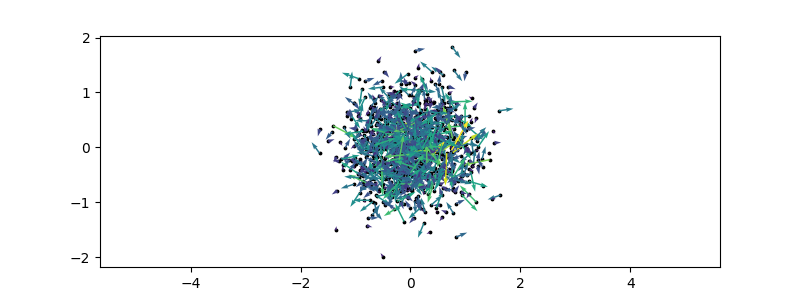
\includegraphics[width=0.5\linewidth]{tcc//img/1000corpos_E_negativa.png}
        \caption{Posições e momentos do problema-modelo \ref{probmodelo:1000corpos_energianegativa}.}
        \label{fig:probmodelo_1000corpos_E_negativa}
    \end{figure}
\end{probmodelo}

\begin{probmodelo}[1000 corpos e $E=0$]\label{probmodelo:1000corpos_energianula}
    Trata-se de um problema com $N=10^3$, todas as integrais primeiras nulas e massas iguais a $10^{-3}$. As posições e momentos lineares podem ser visualizados na figura \ref{fig:probmodelo_1000corpos_E_nula}.
    \begin{figure}[H]
        \centering
        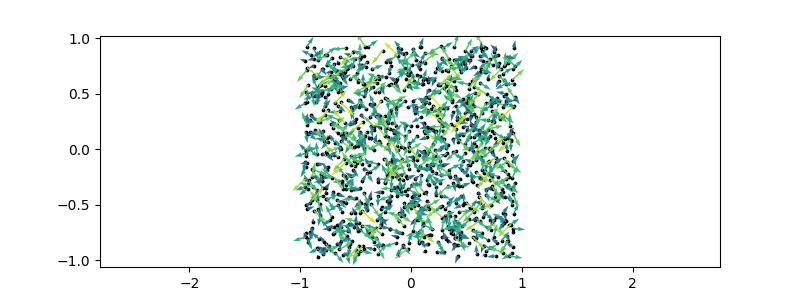
\includegraphics[width=0.5\linewidth]{tcc//img/1000corpos_E_nula.png}
        \caption{Posições e momentos do problema-modelo \ref{probmodelo:1000corpos_energianula}.}
        \label{fig:probmodelo_1000corpos_E_nula}
    \end{figure}
\end{probmodelo}

\begin{probmodelo}[1000 corpos e $E=0.25$ (massas iguais)]\label{probmodelo:1000corpos_energiapositiva_1}
    Trata-se de um problema com $N=10^3$, $E=0.25$, todas as outras integrais primeiras nulas e massas iguais a $10^{-3}$. As posições e momentos lineares podem ser visualizados na figura \ref{fig:probmodelo_1000corpos_E_positiva_1}.
    \begin{figure}[H]
        \centering
        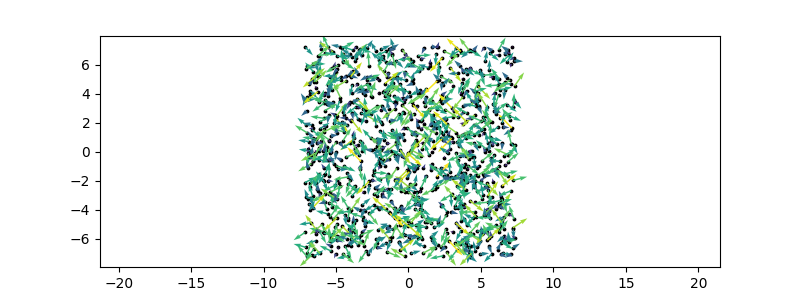
\includegraphics[width=0.5\linewidth]{tcc//img/1000corpos_E_positiva_1.png}
        \caption{Posições e momentos do problema-modelo \ref{probmodelo:1000corpos_energiapositiva_1}.}
        \label{fig:probmodelo_1000corpos_E_positiva_1}
    \end{figure}
\end{probmodelo}

\begin{probmodelo}[1000 corpos e $E=0.25$ (massas diferentes)]\label{probmodelo:1000corpos_energiapositiva_2}
    Trata-se de um problema com $N=10^3$, $E=0.25$, todas as outras integrais primeiras nulas e massas diferentes. As posições e momentos lineares podem ser visualizados na figura \ref{fig:probmodelo_1000corpos_E_positiva_2}.
    \begin{figure}[H]
        \centering
        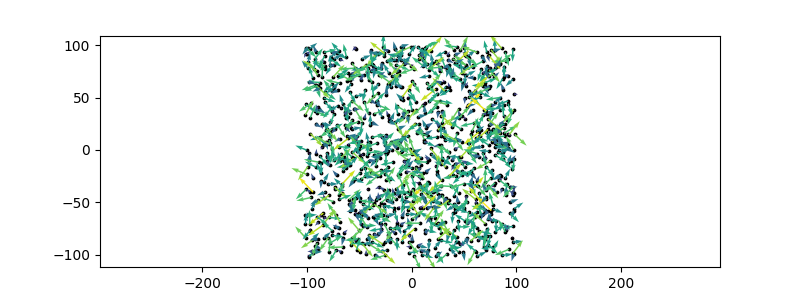
\includegraphics[width=0.5\linewidth]{tcc//img/1000corpos_E_positiva_2.png}
        \caption{Posições e momentos do problema-modelo \ref{probmodelo:1000corpos_energiapositiva_2}.}
        \label{fig:probmodelo_1000corpos_E_positiva_2}
    \end{figure}
\end{probmodelo}

\chapter{Demonstrações de propriedades da Dinâmica de Formas}\label{apendice:demonstracoes_dinamica_de_formas}

Em vias de facilitar a leitura e compreensão da teoria da Dinâmica de Formas para o PNCG, algumas demonstrações não foram apresentadas no corpo do texto. Porém, como tratam-se de resultados importantes para a teoria e cuja demonstração não foi publicada na literatura, vale apresentá-las neste apêndice.

\begin{proposition}[Equação \ref{eq:new_constraints}]\label{prop:new_constraints}
    Para as coordenadas objetivas $(\vet \sigma, \vet \pi)$, valem as propriedades
    \begin{align}
        \sum_{a=1}^N \vet \sigma_a \cdot \vet \sigma_a = 1, \quad
        \sum_{a=1}^N \vet \pi^a \cdot \vet \sigma_a = 0, \nonumber \\
        \sum_{a=1}^N \sqrt{m_a} \vet \sigma_a = 0, \quad
        \sum_{a=1}^N \sqrt{m_a} \vet \pi^a = 0.
    \end{align}
\end{proposition}
\begin{Proof}
    \begin{flalign*}
        \sum_{a=1}^{N} \vet \sigma_a \cdot \vet \sigma_a
        = \dfrac{1}{R^2} \sum_{a=1}^{N} m_a \vet q_a \cdot \vet q_a
        = \dfrac{R^2}{R^2} = 1.&&
    \end{flalign*}
    \begin{flalign*}
        \sum_a \vet \pi^a \cdot \vet \sigma_a
        = \dfrac{\cancel R}{D_0} \dfrac{1}{\cancel R} \sum_a \dfrac{\vet p^a_{cm}}{\cancel{\sqrt{m_a}}} \cancel{\sqrt{m_a}} \vet q_a^{cm} - \dfrac{D}{D_0} \sum_a \vet \sigma_a \cdot \vet \sigma_a
        = \dfrac{D}{D_0} - \dfrac{D}{D_0} = 0.&&
    \end{flalign*}
    \begin{flalign*}
        \sum_a \sqrt{m_a} \vet \sigma_a 
        = \dfrac{1}{R} \sum_a m_a \vet q_a
        = \dfrac{1}{R} \sum_a m_a \vet q_a
        = \vet 0.&&
    \end{flalign*}
    \begin{flalign*}
        \sum_a \sqrt{m_a} \vet \pi^a 
        = \dfrac{R}{D_0} \sum_a \dfrac{\sqrt{m_a}}{\sqrt{m_a}}\vet p^a - \dfrac{D}{D_0} \sum_a \sqrt{m_a} \vet \sigma_a
        = \vet 0.&&
    \end{flalign*}
\end{Proof}

\begin{proposition}[Invariância por escala, equação \ref{eq:invariancia_por_escala}]\label{prop:invariancia_por_escala}
    As coordenadas objetivas $(\vet \pi, \vet \sigma)$ são invariantes por escala, pois comutam com $D$ e com $R$,
    \begin{equation*}
        \{ f(D, R), \vet \pi_a \} = \{ f(D,R), \vet \sigma_a \} = 0.
    \end{equation*}
\end{proposition}
\begin{Proof}
    Primeiro, observe que $\vet x$ comutar com $f(D, R)$ equivale a $\vet x$ comutar com $D$ e com $R$:
    \begin{align*}
        \{ f(D,R), \vet x \}
        &= \sum_a \derpar{f(D,R)}{\vet q_a} \cdot \derpar{\vet x}{\vet p^a} - \derpar{f(D,R)}{\vet p^a} \cdot \derpar{\vet x}{\vet q_a} 
        \\
        &= \sum_a \left[ \derpar{f}{D} \derpar{D}{\vet q_a} + \derpar{f}{R} \derpar{R}{\vet q_a} \right] \derpar{\vet x}{\vet p^a} - \left[ \derpar{f}{D} \derpar{D}{\vet p^a} + \derpar{f}{R} \derpar{R}{\vet p^a} \right] \derpar{\vet x}{\vet q_a}
        \\
        &= \derpar{f}{D} \sum_a \left[\derpar{D}{\vet q_a} \derpar{\vet x}{\vet p^a} - \derpar{D}{\vet p^a} \derpar{\vet x}{\vet q_a} \right] + \derpar{f}{R} \sum_a \left[\derpar{R}{\vet q_a} \derpar{\vet x}{\vet p^a} - \derpar{R}{\vet p^a} \derpar{\vet x}{\vet q_a} \right] 
        \\
        &= \derpar{f}{D} \{D, \vet x\} + \derpar{f}{R} \{R, \vet x\}.
    \end{align*}
    Assim, basta verificar as comutatividades individuais. Temos as derivadas parciais:
    \begin{align*}
        \derpar{\vet \sigma_a}{\vet q_b} = \dfrac{\sqrt{m_a}}{R^2}\left(\delta_a^b R - \dfrac{m_b}{R} \vet q_a \cdot \vet q_b\right),
        \quad
        \derpar{\vet \sigma_a}{\vet p_b} = 0,
        \quad
        \derpar{\vet \pi^a}{\vet p_b} = \dfrac{R}{\sqrt m_a} \delta_a^b - \vet q_b \cdot \vet \sigma_a,
        \\
        \derpar{\vet \pi^a}{\vet q_b} = \dfrac{m_b}{\sqrt{m_a}} R  \vet p^a \cdot \vet q_b - \vet p^a \cdot \vet \sigma_a - \dfrac{D \sqrt{m_a}}{R^2} \left( \delta_a^b R - \dfrac{m_b}{R} \vet q_a \cdot \vet q_b \right).
    \end{align*}
    Então:
    \begin{flalign*}
        \{D, \vet \sigma_a \} 
        &= \sum_i \vet p^i \derpar{\vet \sigma_a}{\vet p^i} - \vet r_i \derpar{\vet \sigma_a}{\vet r_i}
        = - \sum_i \vet r_i \dfrac{\sqrt{m_a}}{R^2}\left( \delta_a^i R - \dfrac{m_i}{R} \vet q_a \cdot \vet r_i \right)&&
        \\
        &= - \dfrac{\sqrt{m_a}}{R} \vet q_a + \dfrac{\sqrt{m_a}}{R} \vet q_a \sum_i \dfrac{m_i \vet r_i \cdot \vet r_i}{R^2} 
         = - \dfrac{\sqrt{m_a}}{R} \vet q_a + \dfrac{\sqrt{m_a}}{R} \vet q_a \sum_i \vet \sigma_i \cdot \vet \sigma_i = 0.&&
    \end{flalign*}
    \begin{flalign*}
        \{R, \vet \sigma_a \} = 
        \sum_i \derpar{R}{\vet r_i} \derpar{\vet \sigma_a}{\vet p^i} - \derpar{R}{\vet p^i} \derpar{\vet \sigma_a}{\vet r_i} = 0.&&
    \end{flalign*}
    \begin{flalign*}
        \{D, \vet \pi^a \} 
        &= \sum_i \vet p^i \left( \dfrac{R}{\sqrt{m_a}}\delta_a^i - \vet r_i \vet \sigma_a \right) - \vet r_i \derpar{\vet \pi_a}{\vet q_i} 
        = \vet \pi^a - \dfrac{R}{\sqrt{m_a}} \vet p^a \sum_i \norma{\vet \sigma_i}^2 - \dfrac{D\sqrt{m_a}}{R} \vet q_a \sum_i \norma{\sigma_i}^2 &&
        \\ 
        &= \vet \pi^a - \dfrac{R}{\sqrt{m_a}} \vet p^a - \dfrac{D \sqrt{m_a}}{R} \vet q_a
        = \vet \pi^a - \vet \pi^a = 0. &&
    \end{flalign*}
    \begin{flalign*}
        \{R, \vet \pi^a\} 
        &= \sum_i \derpar{R}{\vet r_i} \derpar{\vet \pi^a}{\vet p^i} - \derpar{R}{\vet p^i}\derpar{\vet \pi^a}{\vet r_i}
         = \sum_i \dfrac{m_i \vet r_i}{R} \left( \dfrac{R}{\sqrt{m_a}} \delta_a^i - \vet r_i \vet \sigma_a \right) &&
         \\
        &= \sqrt{m_a} \vet q_a - \vet \sigma_a \sum_i \dfrac{m_i \vet r_i \vet r_i}{R}
         = \sqrt{m_a} \vet q_a - R \vet \sigma_a \sum_i \norma{\vet \sigma_i}^2 &&
         \\
        &= R(\vet \sigma_a - \vet \sigma_a) = 0.&&
    \end{flalign*}
    Assim, obtivemos que
    \begin{equation*}
        \{D, \vet \sigma_a\} = \{D, \vet \pi^a \} = \{R, \vet \sigma_a\} = \{R, \vet \pi^a\} = 0.
    \end{equation*}
\end{Proof}

\par

% %%%% Anexos %%%%

% \makeatletter
% \if@openright\cleardoublepage\else\clearpage\fi
% \makeatother

% \pagestyle{appendix} % repete o anterior, caso você não use apêndices

% \annex

% % \addappheadtotoc acrescenta a palavra "Anexo" ao sumário; se
% % só há anexos, sem apêndices, provavelmente não é necessário.
% \addappheadtotoc

% \par